\documentclass[6pt,a4paper]{extarticle}
\usepackage[UTF8,fontset=none]{ctex}
\setCJKmainfont{Songti SC}
\setCJKsansfont{Heiti SC}
\setCJKmonofont{Songti SC}
\usepackage[a4paper,margin=0.7cm]{geometry}
\usepackage{amsmath,amssymb,bm}
\usepackage{multicol}
\usepackage{graphicx}
\usepackage{enumitem}
\usepackage{titlesec}
\usepackage{mathtools}

\pagestyle{empty}
\setlength{\parindent}{0pt}
\setlength{\parskip}{1pt}
\setlength{\columnsep}{0.4cm}
\setlength{\columnseprule}{0.2pt}
\setlength{\abovedisplayskip}{1.5pt}
\setlength{\belowdisplayskip}{1.5pt}
\setlength{\abovedisplayshortskip}{1pt}
\setlength{\belowdisplayshortskip}{1pt}
\setlist{nosep,leftmargin=1.2em,itemsep=0pt,parsep=0pt,topsep=0pt}
\titleformat{\section}{\bfseries\sffamily\small}{}{0pt}{}[\vspace{-3pt}\hrule]
\titleformat{\subsection}{\bfseries\sffamily\footnotesize}{}{0pt}{}
\titlespacing*{\section}{0pt}{2pt}{1pt}
\titlespacing*{\subsection}{0pt}{1.5pt}{0.5pt}

\newcommand{\key}[1]{\textbf{#1}}

\begin{document}
\fontsize{7.4pt}{8.7pt}\selectfont
\begin{multicols}{3}
\raggedcolumns

\section{线性代数}
二阶行列式：主对角线乘积减去副对角线乘积。

三阶行列式：把前两列抄到右边，三条正对角线方向乘积取正，三条副对角线乘积取负。

矩阵求逆：
$$A^{-1}=\frac{1}{\det A}\mathrm{adj}(A),\quad \mathrm{adj}(A)_{ij}=(-1)^{i+j}M_{ji}$$
其中 $M_{ji}$ 是去掉第 $j$ 行第 $i$ 列的余子式（注意下标转置）。

\section{贝叶斯决策}
分两步：(1) 算出不同猜测的可能性大小，即计算后验概率；(2) 根据准则决定最可靠的策略。

后验概率
$$P(\theta\mid D)=\frac{P(D\mid\theta)P(\theta)}{P(D)}$$
\begin{itemize}
\item $D$ 一般是连续变量；$\theta$ 是离散变量，可看作类别。
\item $P(\theta)$ 先验概率：依据大量统计数据确定某类事物出现的比例。
\item $P(X|\omega)$ 类条件概率密度：同一事物的各个属性有一定变化范围，在该范围内的分布密度用一种函数形式表示。例：$P(x{=}38|y{=}w_1)=0.16$。
\end{itemize}
\begin{center}
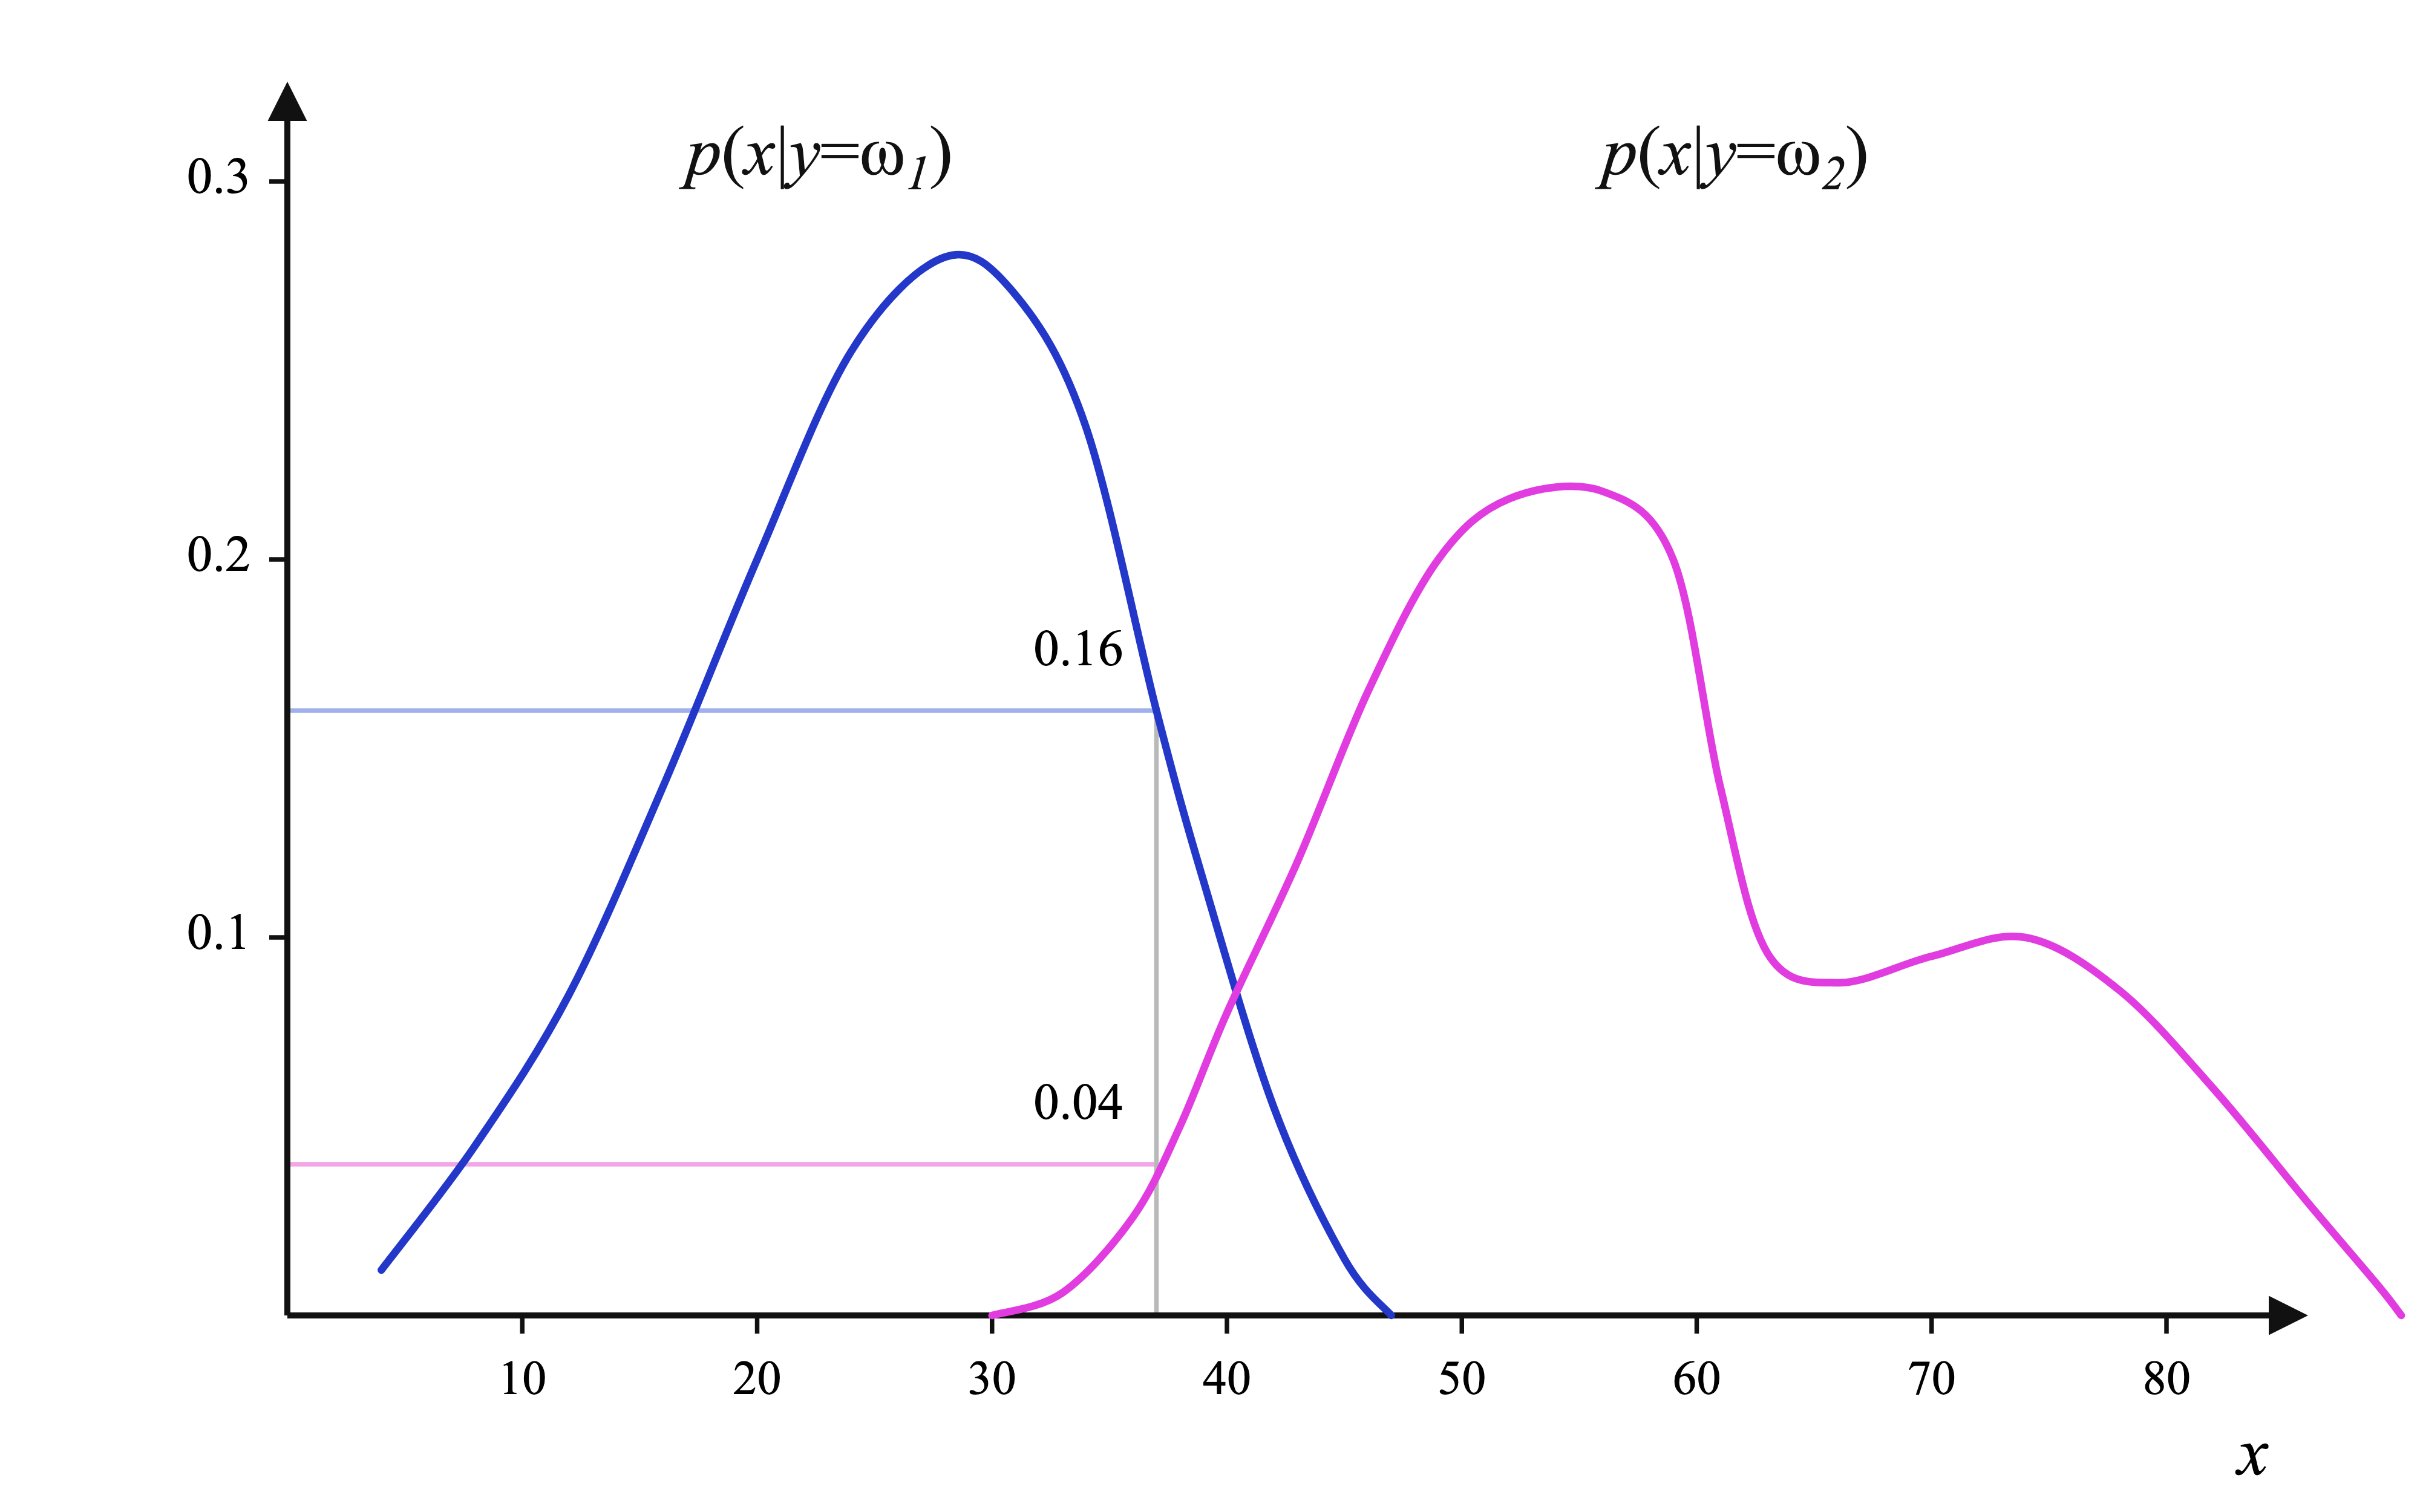
\includegraphics[width=0.55\linewidth]{模式识别/imgs/image-20261107162344482.png}
\end{center}

\subsection{决策规则}
\textbf{1. 基于最小错误概率的贝叶斯决策}：选择\key{后验概率}最大的类别（依赖先验概率，属不确定性推理）。
\begin{enumerate}[label=(\arabic*)]
\item 后验概率形式：$P(\omega_i|x)=\max_j P(\omega_j|x)\Rightarrow x\in\omega_i$
\item 条件概率形式：$P(x|\omega_i)P(\omega_i)>P(x|\omega_j)P(\omega_j),\ \forall j\ne i\Rightarrow x\in\omega_i$
\item 似然比形式：$\dfrac{P(x|\omega_i)}{P(x|\omega_j)}>\dfrac{P(\omega_j)}{P(\omega_i)},\ \forall j\ne i\Rightarrow x\in\omega_i$
\item 对数形式：$\ln P(x|\omega_i)+\ln P(\omega_i)>\ln P(x|\omega_j)+\ln P(\omega_j),\ \forall j\ne i\Rightarrow x\in\omega_i$
\end{enumerate}
\textbf{2. 最小风险贝叶斯决策}：各种错误造成的损失不同，选条件风险最小的动作。
\begin{enumerate}[label=(\arabic*)]
\item 决策表见下图。损失函数 $\lambda(\alpha_i,\omega_j)$：真实状态为 $\omega_j$ 而采取决策 $\alpha_i$ 时的损失（把属于 $\omega_j$ 的样本归到 $i$ 类）。
\item 条件风险（条件期望损失）：$R(\alpha_i|x)=E[\lambda(\alpha_i,\omega_j)]=\sum_{j=1}^{c}\lambda(\alpha_i,\omega_j)P(\omega_j|x),\ i=1,\ldots,a$
\item 两分类：
$\begin{aligned}R(\alpha_1|x)&=\lambda_{11}P(\omega_1|x)+\lambda_{12}P(\omega_2|x)\\R(\alpha_2|x)&=\lambda_{21}P(\omega_1|x)+\lambda_{22}P(\omega_2|x)\end{aligned}$
转换得 $\dfrac{p(x|w_1)}{p(x|w_2)}>\dfrac{(\lambda_{12}-\lambda_{22})P(w_2)}{(\lambda_{21}-\lambda_{11})P(w_1)}$
\item 0-1 损失：$\lambda=\begin{cases}0,&i=j\\1,&i\ne j\end{cases}$，$i,j=1,\ldots,c$ 时，最小风险决策与最小错误率决策等价。
\end{enumerate}
\begin{center}
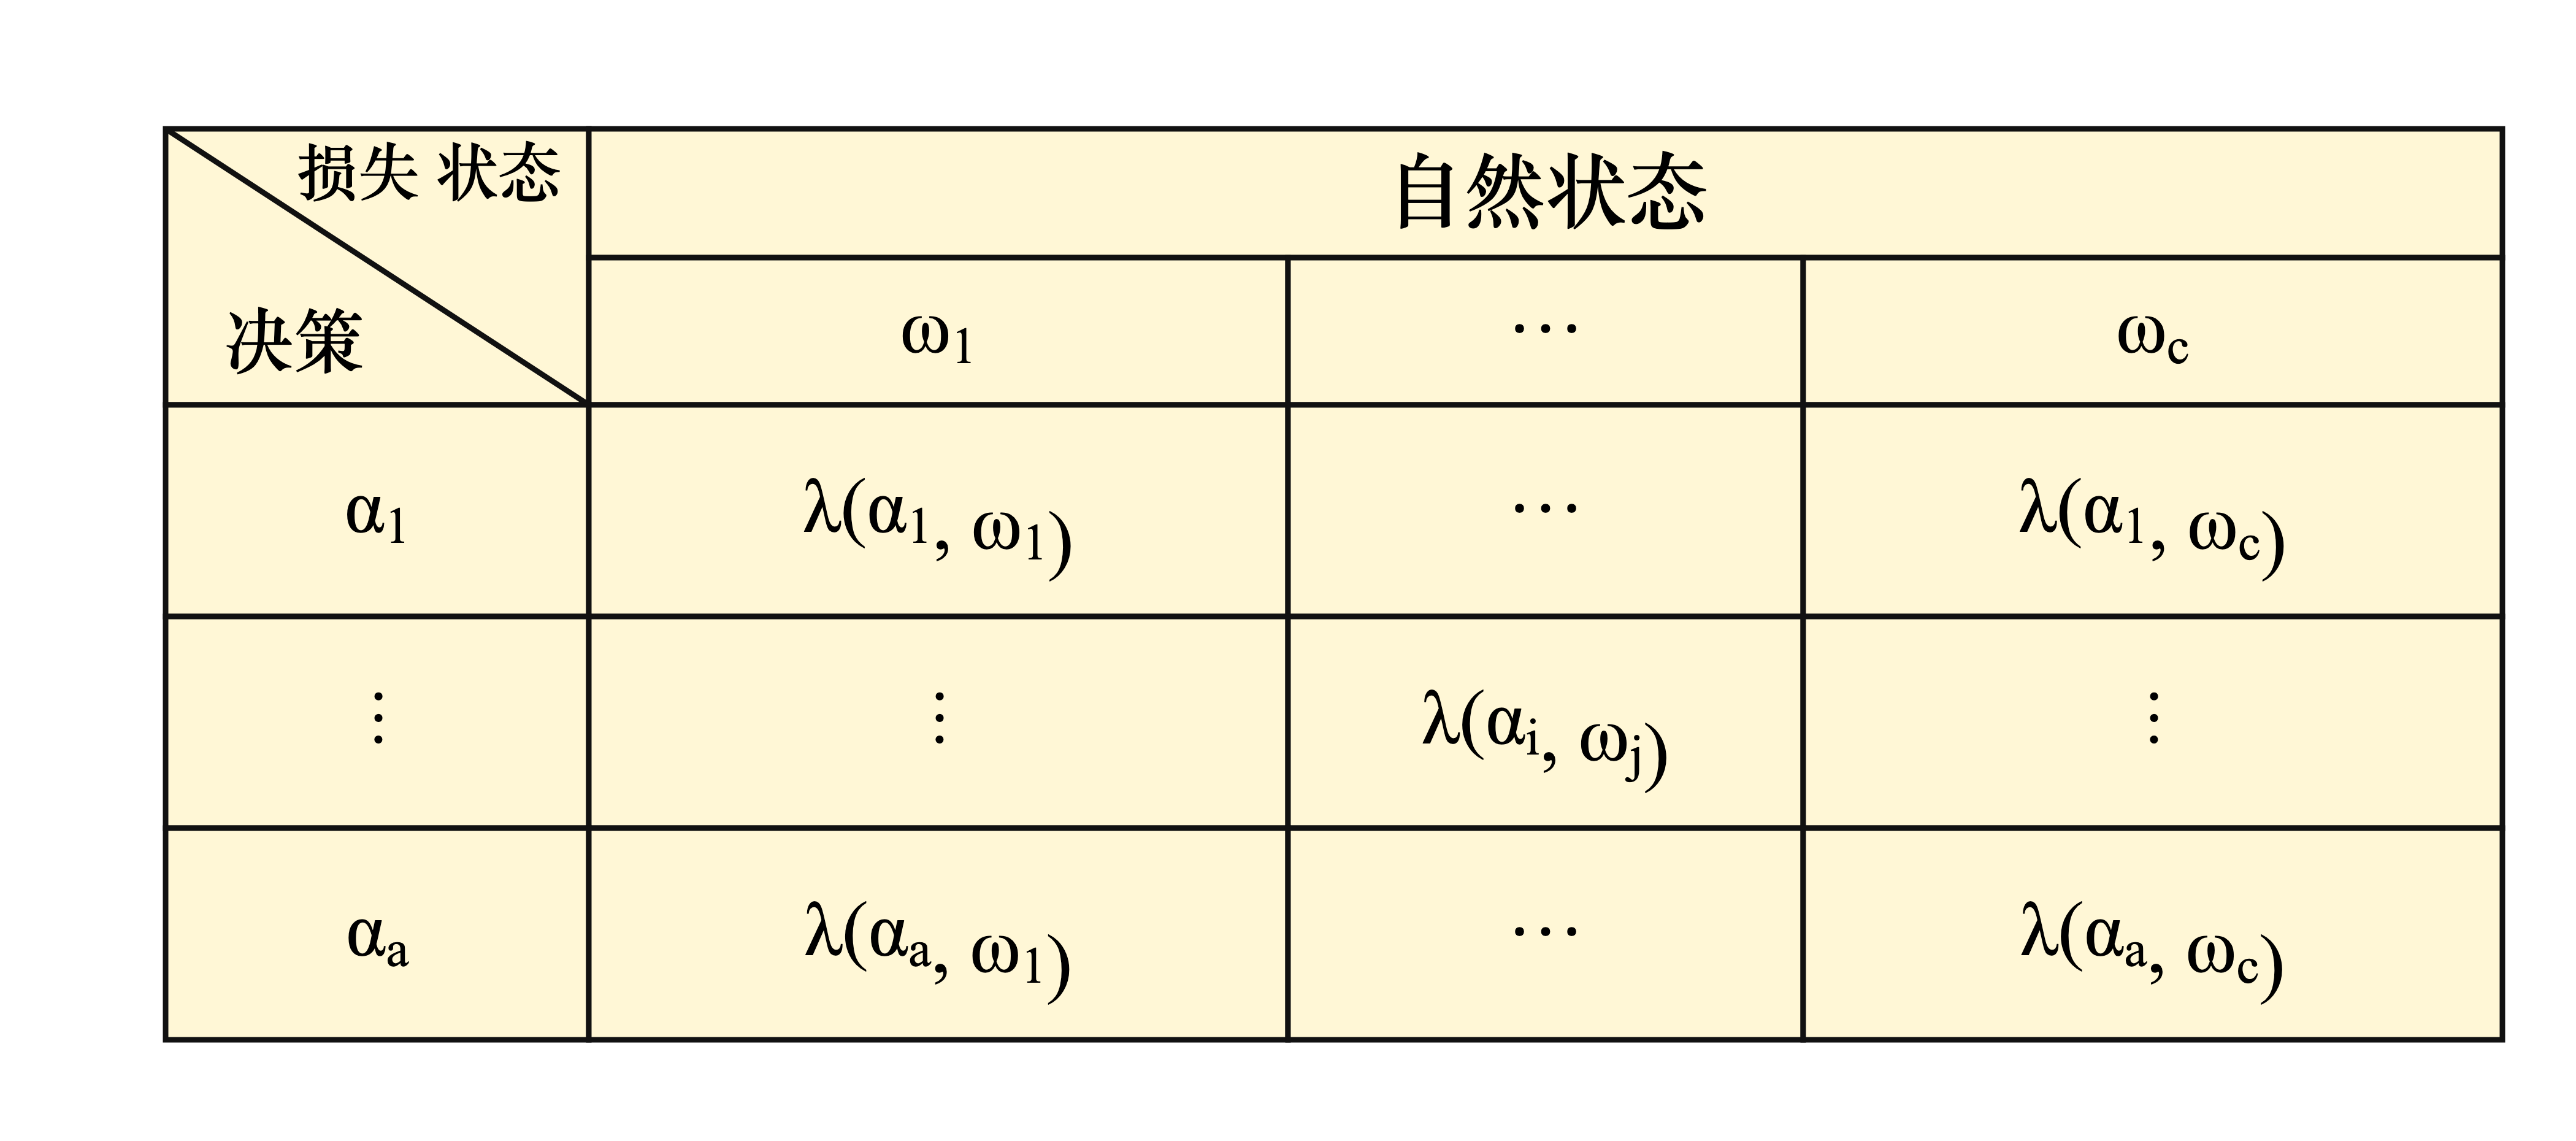
\includegraphics[width=0.6\linewidth]{模式识别/imgs/image-20261107163557118.png}
\end{center}

\subsection{判别函数}
\key{决策域}：待识别特征向量落在哪个决策域，就判为哪一类。\key{决策面}：决策域的边界（一维点，二维线，三维面）。\key{判别函数}：表达决策规则的函数，后验概率和条件风险都是判别函数。

两类情况下可定义
$$\begin{aligned}
\text{(1)}\ g(x)&=P(\omega_1|x)-P(\omega_2|x)\\
\text{(2)}\ g(x)&=p(x|\omega_1)P(\omega_1)-p(x|\omega_2)P(\omega_2)\\
\text{(3)}\ g(x)&=\ln\frac{p(x|\omega_1)}{p(x|\omega_2)}-\ln\frac{P(\omega_2)}{P(\omega_1)}
\end{aligned}$$
决策面方程 $g(x)=0$，如 $P(\omega_1|x)-P(\omega_2|x)=0$。

\subsection{正态分布下的决策}
假定类条件概率密度服从正态分布
$$\begin{aligned}
p(x)&=\frac{1}{\sqrt{2\pi}\sigma}e^{-\frac{(x-\mu)^2}{2\sigma^2}},\ \text{记作 }N(\mu,\sigma^2)\\
\mu&=E\{x\}=\int_{-\infty}^{+\infty}x\,p(x)dx\\
\sigma^2&=\int_{-\infty}^{+\infty}(x-\mu)^2p(x)dx
\end{aligned}$$
$$\begin{aligned}
\mathbf{x}&=[x_1,\ldots,x_d]^T\\
p(\mathbf{x})&=\frac{1}{(2\pi)^{d/2}|\Sigma|^{1/2}}e^{-\frac12(\mathbf{x}-\bm\mu)^T\Sigma^{-1}(\mathbf{x}-\bm\mu)}\\
\bm\mu&=E\{\mathbf{x}\}=[\mu_1,\ldots,\mu_d]^T\ \text{（均值向量）}
\end{aligned}$$
判别函数
$$\begin{aligned}
g_i(\mathbf{x})&=\ln p(\mathbf{x}|\omega_i)+\ln P(\omega_i)\\
&=-\tfrac12(\mathbf{x}-\bm\mu_i)^T\Sigma_i^{-1}(\mathbf{x}-\bm\mu_i)\\
&\quad-\tfrac d2\ln2\pi-\tfrac12\ln|\Sigma_i|+\ln P(\omega_i)
\end{aligned}$$
决策面方程
$$\begin{aligned}
&-\tfrac12\big[(\mathbf{x}-\bm\mu_i)^T\Sigma_i^{-1}(\mathbf{x}-\bm\mu_i)\\
&\ -(\mathbf{x}-\bm\mu_j)^T\Sigma_j^{-1}(\mathbf{x}-\bm\mu_j)\big]\\
&-\tfrac12\ln\frac{|\Sigma_i|}{|\Sigma_j|}+\ln\frac{P(\omega_i)}{P(\omega_j)}=0
\end{aligned}$$

\section{参数估计}
\subsection{概率密度函数估计}
后验概率依赖先验概率和类条件概率，二者通常未知，已知的只有有限数目的样本。先验概率可用各类出现的频率估计；类条件概率包含随机变量的全部信息，无法靠经验得到，一般假定为多元正态分布，问题转为估计参数 $\mu$ 和 $\Sigma_i$。

基本估计方法分参数估计和非参数估计，参数估计有\key{最大似然估计}和\key{贝叶斯估计}。最大似然估计：模型已确定但参数未知，利用结果反推。

\subsection{最大似然估计}
MLE 把参数视为固定但未知的量，选择使已观测训练样本出现概率最大的参数值。设 $D=\{x_1,\ldots,x_N\}$ 独立同分布，$p(x_n|\theta)$ 为样本分布，似然函数
$$L(\theta;D)=p(D|\theta)=\prod_{n=1}^{N}p(x_n|\theta)$$
通常最大化对数似然（与最大化似然等价）：
$$\ell(\theta;D)=\ln L(\theta;D)=\sum_{n=1}^{N}\ln p(x_n|\theta)$$
对 $\ell$ 关于参数求梯度并令其为零，解出参数：
$$\nabla_\theta\ell(\theta;D)=0,\quad \hat\theta_{\rm ML}=\arg\max_\theta L(\theta;D)$$
\textbf{高斯分布的 MLE}：$x_1,\ldots,x_N$ 来自 $N(\mu,\sigma^2)$。
\begin{itemize}
\item 只估计均值（方差已知）：$\hat\mu_{\rm ML}=\bar x=\frac1N\sum_{n=1}^Nx_n$。
\item 均值方差都未知：$\hat\mu_{\rm ML}=\bar x$，$\hat\sigma^2_{\rm ML}=\frac1N\sum_{n=1}^N(x_n-\bar x)^2$。
\end{itemize}
$d$ 维高斯 $N(\bm\mu,\Sigma)$：
$$\begin{aligned}\hat{\bm\mu}_{\rm ML}&=\frac1N\sum_{n=1}^N\mathbf{x}_n\\ \hat\Sigma_{\rm ML}&=\frac1N\sum_{n=1}^N(\mathbf{x}_n-\hat{\bm\mu}_{\rm ML})(\mathbf{x}_n-\hat{\bm\mu}_{\rm ML})^T\end{aligned}$$

\subsection{贝叶斯估计}
通过贝叶斯决策得到参数 $\theta$ 的最优估计，使总期望风险最小。
\begin{enumerate}
\item 确定参数 $\theta$ 的先验分布。
\item 由样本集 $D$ 求样本联合分布 $p(D|\theta)=\prod_{n=1}^Np(x_n|\theta)$。
\item 由贝叶斯公式求后验概率 $p(\theta|D)=\dfrac{p(D|\theta)P(\theta)}{\int p(D|\theta)P(\theta)d\theta}$。
\item 求贝叶斯估计量 $\hat\theta=\int_\theta\theta\,p(\theta|D)d\theta$。
\end{enumerate}
给定 $D$，$x\sim N(\mu,\sigma^2)$，均值未知、方差已知。

(1) 均值的先验分布：$\mu\sim N(\mu_0,\sigma_0^2)$。

(2) 求后验 $p(\mu|D)$：
$$p(\mu|D)=\frac{p(D|\mu)p(\mu)}{p(D)}=\alpha\,p(D|\mu)p(\mu)$$
其中 $\alpha$ 吸收所有与 $\mu$ 无关的项。
$$\begin{aligned}
p(\mu|D)&=\alpha\prod_{i=1}^N\tfrac{1}{\sqrt{2\pi}\sigma}e^{-\frac12\frac{(x_i-\mu)^2}{\sigma^2}}\\
&\quad\cdot\tfrac{1}{\sqrt{2\pi}\sigma_0}e^{-\frac12\frac{(\mu-\mu_0)^2}{\sigma_0^2}}\\
&=\alpha'\exp\Big(-\tfrac12\Big(\sum_{i=1}^N\tfrac{(x_i-\mu)^2}{\sigma^2}\\
&\quad+\tfrac{(\mu-\mu_0)^2}{\sigma_0^2}\Big)\Big)\\
&=\alpha''\exp\Big(-\tfrac12\Big[\Big(\tfrac N{\sigma^2}+\tfrac1{\sigma_0^2}\Big)\mu^2\\
&\quad-2\Big(\tfrac1{\sigma^2}\sum_{i=1}^Nx_i+\tfrac{\mu_0}{\sigma_0^2}\Big)\mu\Big]\Big)\\
&=\tfrac{1}{\sqrt{2\pi}\sigma_N}\exp\Big(-\tfrac12\tfrac{(\mu-\mu_N)^2}{\sigma_N^2}\Big)
\end{aligned}$$
故 $p(\mu|D)\sim N(\mu_N,\sigma_N^2)$。比较指数项系数得
$$\begin{cases}
\dfrac1{\sigma_N^2}=\dfrac N{\sigma^2}+\dfrac1{\sigma_0^2}\\[4pt]
\dfrac{\mu_N}{\sigma_N^2}=\dfrac1{\sigma^2}\hat\mu_N+\dfrac{\mu_0}{\sigma_0^2}
\end{cases}\quad \hat\mu_N=\frac1N\sum_{i=1}^Nx_i$$
解得
$$\boxed{\begin{aligned}
\mu_N&=\frac{N\sigma_0^2}{N\sigma_0^2+\sigma^2}\hat\mu_N+\frac{\sigma^2}{N\sigma_0^2+\sigma^2}\mu_0\\
\sigma_N^2&=\frac{\sigma^2\sigma_0^2}{N\sigma_0^2+\sigma^2}
\end{aligned}}$$
$\mu$ 的贝叶斯估计值即 $\mu$ 的期望：
$$\hat\mu=\int\mu\,p(\mu|D)d\mu=\mu_N$$
因此
$$\boxed{\hat\mu=\frac{N\sigma_0^2}{N\sigma_0^2+\sigma^2}\hat\mu_N+\frac{\sigma^2}{N\sigma_0^2+\sigma^2}\mu_0}$$
\end{multicols}
\end{document}
